\section{ПРОЄКТУВАННЯ СИСТЕМИ ДІАЛОГОВОЇ ВЗАЄМОДІЇ З LLM}

\subsection{Вибір архітектури програмної системи}

Для розробки системи діалогової взаємодії з LLM обрано модульну багаторівневу архітектуру. Такий підхід дозволяє розділити відповідальність між окремими компонентами системи та забезпечити можливість подальшого розширення без істотної зміни існуючого коду.

Загальна архітектура системи складається з таких рівнів:
\begin{itemize}
  \item рівень користувацької взаємодії;
  \item рівень бізнес-логіки;
  \item рівень збереження даних;
  \item рівень взаємодії з мовною моделлю;
  \item рівень конфігурації та допоміжних сервісів.
\end{itemize}

Рівень користувацької взаємодії представлений web-інтерфейсом і CLI-режимом. Рівень бізнес-логіки реалізовано у компоненті \texttt{ChatManager}. Рівень збереження даних реалізовано через \texttt{PostgresStorage}, а рівень взаємодії з мовною моделлю --- через \texttt{BaseLLMService}, \texttt{TransformersLLMService}, \texttt{UnavailableLLMService} та \texttt{LLMRuntime}.

\begin{figure}[H]
\centering
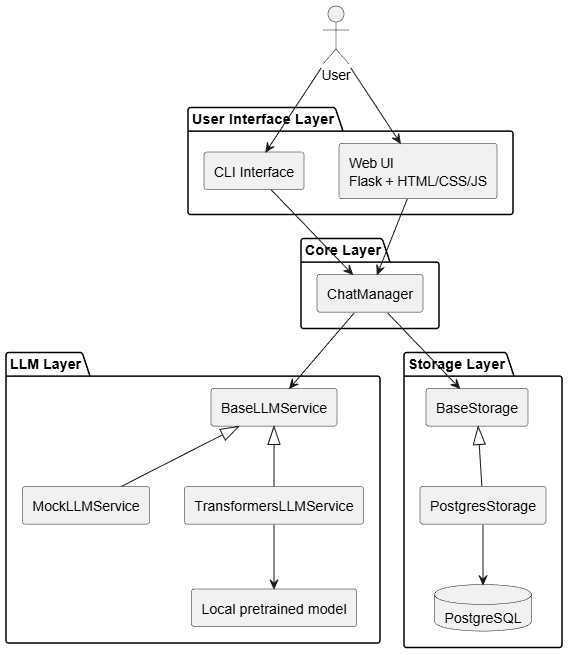
\includegraphics[width=0.8\textwidth]{media/architecture.png}
\caption{Загальна архітектура системи}
\label{fig:architecture}
\end{figure}

\subsection{Формування функціональних і нефункціональних вимог}

На основі технічного завдання та аналізу предметної області сформовано функціональні та нефункціональні вимоги до системи.

\begin{longtable}{|p{1.5cm}|p{13.5cm}|}
\caption{Функціональні вимоги до системи}
\label{tab:functional-requirements}\\
\hline
\textbf{Код} & \textbf{Вимога} \\
\hline
\endfirsthead
\hline
\textbf{Код} & \textbf{Вимога} \\
\hline
\endhead
F1 & Система повинна запускатися з головного файла \texttt{app.py}. \\
\hline
F2 & Система повинна підтримувати web-режим роботи. \\
\hline
F3 & Система повинна підтримувати CLI-режим роботи через параметр \texttt{-t}. \\
\hline
F4 & Користувач повинен мати можливість створювати новий чат. \\
\hline
F5 & Користувач повинен мати можливість відкривати наявний чат. \\
\hline
F6 & Користувач повинен мати можливість перейменовувати чат. \\
\hline
F7 & Користувач повинен мати можливість видаляти чат. \\
\hline
F8 & Користувач повинен мати можливість надсилати повідомлення. \\
\hline
F9 & Система повинна генерувати відповідь через підключений LLM-backend. \\
\hline
F10 & Система повинна зберігати історію чатів і повідомлень у PostgreSQL. \\
\hline
F11 & Система повинна коректно повідомляти про помилки завантаження моделі. \\
\hline
F12 & Система повинна підтримувати Transformers-backend для локальної pretrained-моделі. \\
\hline
F13 & Система повинна відображати Markdown, блоки коду та математичні формули у відповідях асистента. \\
\hline
F14 & Система повинна показувати активний LLM-backend, назву моделі та preset генерації. \\
\hline
F15 & Система повинна підтримувати runtime-перемикання та вивантаження локальних моделей. \\
\hline
F16 & Система повинна підтримувати streaming generation і зупинку активної генерації. \\
\hline
F17 & Система повинна підтримувати підключення PEFT LoRA/QLoRA-адаптерів. \\
\hline
F18 & Система повинна підтримувати пошук повідомлень і експорт діалогу у Markdown. \\
\hline
\end{longtable}

\begin{longtable}{|p{1.5cm}|p{13.5cm}|}
\caption{Нефункціональні вимоги до системи}
\label{tab:non-functional-requirements}\\
\hline
\textbf{Код} & \textbf{Вимога} \\
\hline
\endfirsthead
\hline
\textbf{Код} & \textbf{Вимога} \\
\hline
\endhead
NF1 & Архітектура системи повинна бути модульною: web-рівень, CLI-рівень, доменна логіка, сховище даних, LLM-рівень і конфігурація мають бути винесені в окремі модулі. \\
\hline
NF2 & Компоненти системи повинні мати слабке зв'язування через абстракції \texttt{BaseStorage} і \texttt{BaseLLMService}; доменна логіка не повинна напряму залежати від Flask, PostgreSQL або Transformers. \\
\hline
NF3 & Система повинна бути придатною до подальшого розширення: додавання нового storage-backend, LLM-backend або конфігурації моделі не повинно вимагати зміни основної логіки \texttt{ChatManager}. \\
\hline
NF4 & Основна бізнес-логіка повинна бути покрита автоматизованими тестами на рівні не менше 70\% production-коду; фактичне покриття становить 77\%, набір тестів містить 105 перевірок. \\
\hline
NF5 & Система повинна коректно обробляти помилки користувача: порожні повідомлення, некоректні або дубльовані назви чатів, відсутні моделі та помилки адаптерів мають повертати контрольоване повідомлення, а не аварійне завершення. \\
\hline
NF6 & Web-інтерфейс повинен бути зручним і зрозумілим: користувач має бачити активний backend, модель, adapter, preset генерації, стан завантаження моделі, кнопку зупинки генерації та кнопки копіювання для блоків коду. \\
\hline
NF7 & Дані чатів повинні зберігатися у структурованому вигляді в таблицях \texttt{chats} і \texttt{messages} з ідентифікаторами чатів, ролями повідомлень, timestamp-ами та порядковим номером повідомлення. \\
\hline
NF8 & Конфігурація системи повинна виконуватися через змінні середовища або \texttt{.env} файл; паролі, локальні моделі та адаптери не повинні додаватися до Git-репозиторію. \\
\hline
NF9 & Система не повинна жорстко залежати від конкретної мовної моделі: доступні моделі мають визначатися через локальний каталог \texttt{models/}, \texttt{model\_config.json}, runtime-перемикання та generation presets. \\
\hline
NF10 & Система повинна підтримувати роботу на персональному комп'ютері з Python 3.10 або вище, PostgreSQL і локальними model artifacts; для великих моделей може використовуватися GPU, але малі моделі можуть запускатися на CPU. \\
\hline
\end{longtable}

\subsection{Матриця трасування вимог}

Для підтвердження повноти реалізації сформовано матрицю трасування, яка пов'язує вимоги з програмними модулями та способом перевірки. Такий підхід дозволяє показати, що функціональні й нефункціональні вимоги не є декларативними, а мають відповідні елементи реалізації та тестування.

\small
\begin{longtable}{|p{2.2cm}|p{5.2cm}|p{7.2cm}|}
\caption{Матриця трасування вимог}
\label{tab:requirements-traceability}\\
\hline
\textbf{Вимога} & \textbf{Модуль реалізації} & \textbf{Перевірка} \\
\hline
\endfirsthead
\hline
\textbf{Вимога} & \textbf{Модуль реалізації} & \textbf{Перевірка} \\
\hline
\endhead
F1--F3 & \texttt{app.py}, \texttt{src/web}, \texttt{src/cli} & Перевірка запуску web-режиму, CLI-режиму та тестування базових web routes. \\
\hline
F4--F8 & \texttt{ChatManager}, web endpoints, storage-рівень & Тести \texttt{chat\_manager} і \texttt{web\_app}: створення, відкриття, перейменування, видалення чатів і надсилання повідомлень. \\
\hline
F9--F12 & \texttt{BaseLLMService}, \texttt{TransformersLLMService}, \texttt{UnavailableLLMService}, \texttt{LLMRuntime} & Тести runtime-станів, побудови prompt-ів, fallback-поведінки та обробки помилок завантаження моделі. \\
\hline
F13 & HTML-шаблони, \texttt{script.js}, Markdown/KaTeX renderer & Ручна browser-перевірка Markdown, code blocks і формул, а також regression-перевірки web-відображення. \\
\hline
F14--F17 & \texttt{LLMRuntime}, \texttt{model\_registry}, \texttt{model\_config.json}, generation presets, PEFT adapter loading & Тести \texttt{llm\_runtime}, \texttt{model\_registry}, \texttt{config\_presets}, \texttt{transformers\_prompting}. \\
\hline
F18 & \texttt{ChatManager}, routes пошуку та експорту & Тести пошуку повідомлень і експорту Markdown у групах \texttt{chat\_manager} та \texttt{web\_app}. \\
\hline
NF1--NF3 & Поділ на \texttt{src/core}, \texttt{src/storage}, \texttt{src/llm}, \texttt{src/web}, \texttt{src/cli} & Перевірка структури коду, використання абстракцій і можливість підстановки fake-реалізацій у тестах. \\
\hline
NF4 & Набір автоматизованих тестів, \texttt{coverage.py} & 105 успішних тестів, production coverage 77\%. \\
\hline
NF5--NF8 & Валідація у \texttt{ChatManager}, web routes, storage factory, \texttt{src/config.py} & Тести помилкових сценаріїв, конфігурації, Alembic-міграцій і storage factory. \\
\hline
NF9--NF10 & \texttt{model\_registry}, runtime-перемикання, локальні model artifacts & Перевірка сканування моделей, читання \texttt{model\_config.json}, перемикання і вивантаження моделей. \\
\hline
\end{longtable}
\normalsize

\subsection{Проєктування основних функціональних модулів}

Програмну систему поділено на такі основні модулі: web-інтерфейс, CLI-інтерфейс, модуль керування чатами, LLM-backend, runtime-керування моделлю, модуль збереження даних і конфігураційний модуль.

Модуль web-інтерфейсу відповідає за взаємодію користувача із системою через браузер. CLI-модуль забезпечує альтернативний текстовий режим роботи. Модуль \texttt{ChatManager} координує операції між інтерфейсами користувача, сховищем даних і LLM-сервісом. LLM-модуль реалізує генерацію відповідей через локальну pretrained-модель. Runtime-модуль керує станом моделі, завантаженням, вивантаженням, streaming-генерацією та зупинкою генерації. Модуль збереження даних використовує PostgreSQL для збереження чатів і повідомлень.

\subsection{Проєктування структури бази даних}

Для збереження історії діалогів використовується реляційна база даних PostgreSQL. Структура бази даних складається з двох основних таблиць: \texttt{chats} і \texttt{messages}.

\begin{longtable}{|p{4cm}|p{4cm}|p{7cm}|}
\caption{Структура таблиці \texttt{chats}}
\label{tab:chats-table}\\
\hline
\textbf{Поле} & \textbf{Тип} & \textbf{Опис} \\
\hline
\endfirsthead
\hline
\textbf{Поле} & \textbf{Тип} & \textbf{Опис} \\
\hline
\endhead
\texttt{id} & TEXT & Унікальний ідентифікатор чату \\
\hline
\texttt{title} & TEXT & Назва чату \\
\hline
\texttt{created\_at} & TIMESTAMPTZ & Дата і час створення чату \\
\hline
\texttt{updated\_at} & TIMESTAMPTZ & Дата і час останнього оновлення чату \\
\hline
\end{longtable}

\begin{longtable}{|p{4cm}|p{4cm}|p{7cm}|}
\caption{Структура таблиці \texttt{messages}}
\label{tab:messages-table}\\
\hline
\textbf{Поле} & \textbf{Тип} & \textbf{Опис} \\
\hline
\endfirsthead
\hline
\textbf{Поле} & \textbf{Тип} & \textbf{Опис} \\
\hline
\endhead
\texttt{id} & BIGSERIAL & Унікальний ідентифікатор повідомлення \\
\hline
\texttt{chat\_id} & TEXT & Ідентифікатор чату, до якого належить повідомлення \\
\hline
\texttt{role} & TEXT & Роль автора повідомлення: \texttt{user} або \texttt{assistant} \\
\hline
\texttt{content} & TEXT & Текст повідомлення \\
\hline
\texttt{timestamp} & TIMESTAMPTZ & Дата і час створення повідомлення \\
\hline
\texttt{position} & INTEGER & Порядковий номер повідомлення в чаті \\
\hline
\end{longtable}

\begin{figure}[H]
\centering
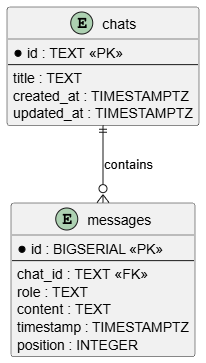
\includegraphics[width=0.5\textwidth]{media/database_er.png}
\caption{ER-діаграма бази даних}
\label{fig:database-er}
\end{figure}

\subsection{UML-діаграма прецедентів}

\begin{figure}[H]
\centering
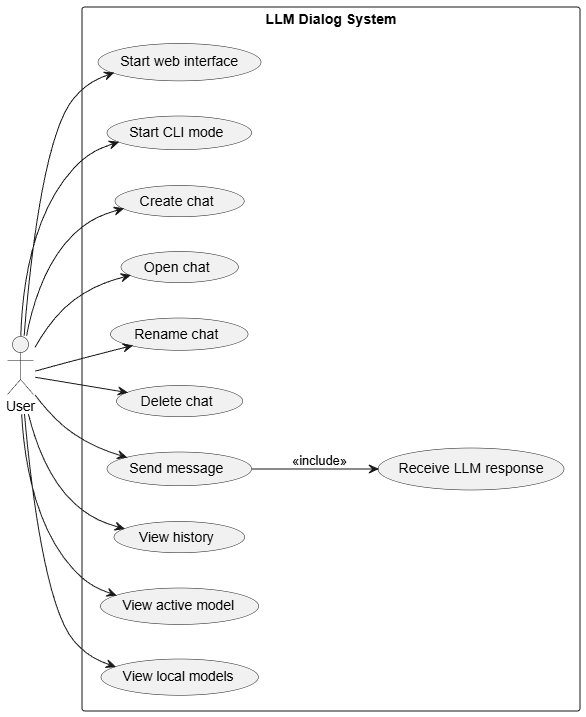
\includegraphics[width=0.8\textwidth]{media/use_case.png}
\caption{UML-діаграма прецедентів системи}
\label{fig:use-case}
\end{figure}

\subsection{UML-діаграма класів}

\begin{figure}[H]
\centering
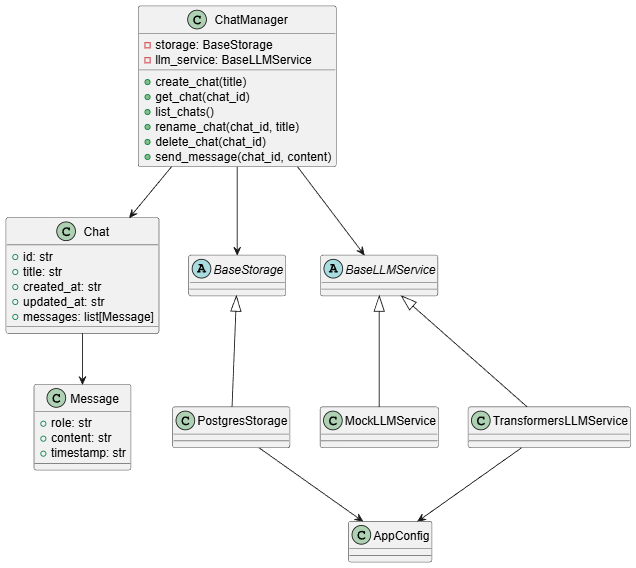
\includegraphics[width=\textwidth]{media/class_diagram.png}
\caption{UML-діаграма класів системи}
\label{fig:class-diagram}
\end{figure}

\subsection{UML-діаграма послідовності}

\begin{figure}[H]
\centering
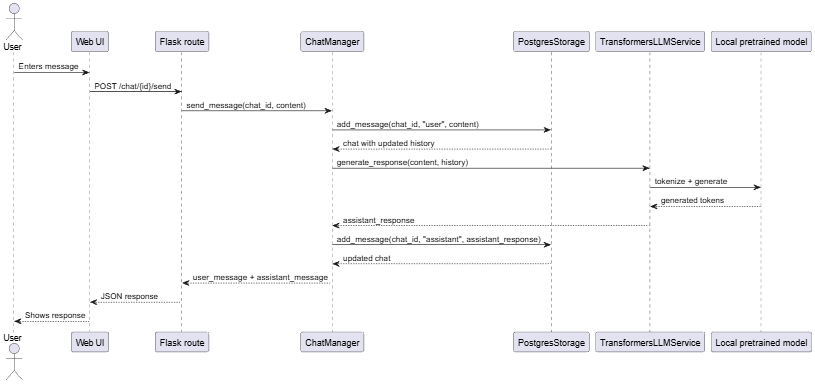
\includegraphics[width=\textwidth]{media/sequence_send_message.png}
\caption{UML-діаграма послідовності надсилання повідомлення}
\label{fig:sequence-send-message}
\end{figure}

\subsection{Опис логічної структури системи}

Логічна структура системи побудована так, щоб окремі частини програмного продукту мали чітко визначені обов'язки. Web-інтерфейс і CLI-інтерфейс не працюють безпосередньо з базою даних або моделлю. Вони звертаються до \texttt{ChatManager}, який координує виконання операцій.

\texttt{ChatManager} не залежить від конкретної реалізації LLM-рівня. Для генерації відповідей використовується інтерфейс \texttt{BaseLLMService}. Для збереження даних у поточній реалізації використовується \texttt{PostgresStorage}, що працює з PostgreSQL.

PostgreSQL використовується як основне сховище даних. Це дозволяє зберігати історію діалогів у структурованому вигляді, підтримувати зв'язок між чатами й повідомленнями та надалі розширювати схему бази даних.

LLM-рівень підтримує Transformers-режим, який дозволяє підключати pretrained-модель, завантажену в локальну директорію \texttt{models/}. Якщо модель не може бути завантажена, використовується \texttt{UnavailableLLMService}, що зберігає інформацію про помилку та дозволяє відобразити її у web-інтерфейсі. Система реалізує потокову генерацію відповідей, зупинку генерації, runtime-перемикання моделей без перезапуску застосунку та підключення LoRA/QLoRA-адаптерів.

Конфігурація системи виконується через змінні середовища або \texttt{.env} файл. Це дозволяє змінювати LLM-backend, модель, preset генерації та параметри підключення до PostgreSQL без зміни вихідного коду.

Таким чином, обрана структура забезпечує модульність, розширюваність, зручність тестування та відповідність поставленим вимогам до курсового проєкту.

\newpage
